\usetikzlibrary{arrows.meta,calc}
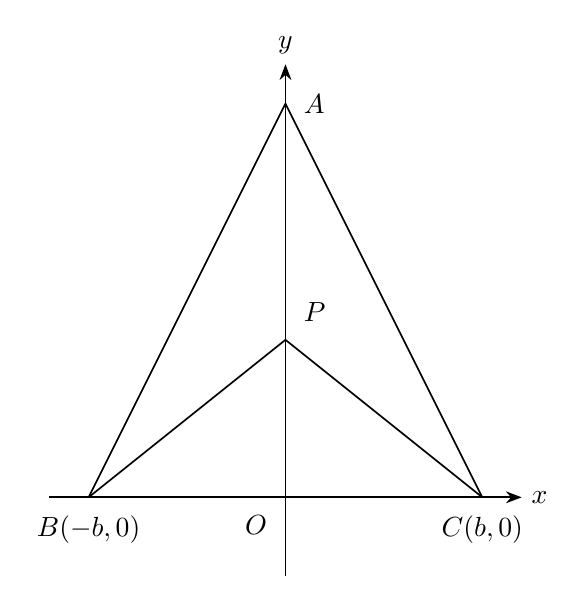
\begin{tikzpicture}[x=1cm,y=1cm,line width=.6pt,font=\normalsize,>=Stealth]
\coordinate (O) at (0,0);
\coordinate (A) at (0,5);
\coordinate (B) at (-2.5,0);
\coordinate (C) at (2.5,0);
\coordinate (P) at (0,2);
\coordinate (XMIN) at (-3,0);
\coordinate (XMAX) at (3,0);
\coordinate (YMIN) at (0,-1);
\coordinate (YMAX) at (0,5.5);
\draw[->] (XMIN)--(XMAX) node[right] {$x$};
\draw[->] (YMIN)--(YMAX) node[above] {$y$};
\draw (A)--(B);
\draw (A)--(C);
\draw (B)--(P);
\draw (C)--(P);
\node[below=3pt] at (B) {$B(-b,0)$};
\node[below=3pt] at (C) {$C(b,0)$};
\node[below left=3pt] at (O) {$O$};
\node[right=3pt] at (A) {$A$};
\node[above right=3pt] at (P) {$P$};
\end{tikzpicture}
